\documentclass[aspectratio=169, 12pt]{beamer}

% --- Packages ---
\usepackage[utf8]{inputenc}
\usepackage{tikz}
\usepackage{amsmath}
\usepackage{booktabs}
\usepackage{xcolor}
\usepackage{algorithm}
\usepackage{algorithmic}
\usetikzlibrary{calc, shapes, patterns, positioning, arrows.meta, backgrounds, decorations.pathreplacing}

% --- Theme ---
\usetheme{Madrid}
\usecolortheme{default}

% Set hidden items to be invisible instead of transparent for cleaner animation
\setbeamercovered{invisible}

% --- Custom Colors ---
\definecolor{job1}{RGB}{70, 130, 180}  % Steel Blue
\definecolor{job2}{RGB}{50, 205, 50}   % Lime Green
\definecolor{job3}{RGB}{220, 20, 60}   % Crimson
\definecolor{idle}{RGB}{200, 200, 200} % Grey

% --- Title Page Data ---
\title[Minimizing Sum of Completion Times]{4.1 Minimizing the Sum of Completion Times \\ on a Single Machine}
% \subtitle{Deterministic Rounding of Linear Programs}
\author[Tanvir (2005014)]{Presenter: Tanvir Hossain \\ Student Id: 2005014}
\date{December 8, 2025}
% \institute{Dept. of CSE}

\begin{document}

% --- Slide 1: Title ---
\begin{frame}
    \titlepage
\end{frame}

% Outline
\begin{frame}{Outline}
    \tableofcontents
\end{frame}

\section{Problem Definition}

% --- Slide 2: The Problem ---
\begin{frame}{The Problem Statement}
    \textbf{Input:} $n$ jobs, each with:
    \begin{itemize}
        \item<2-> Processing time $p_j > 0$ (integer)
        \item<3-> Release date $r_j \geq 0$ (integer)
    \end{itemize}

    \vspace{0.5cm}
    \textbf{Constraints:}
    \begin{itemize}
        \item<4-> Single machine (process one job at a time)
        \item<5-> No job processed before its release date
        \item<6-> Jobs must be processed \textbf{nonpreemptively}
    \end{itemize}

    \vspace{0.5cm}
    \onslide<7->{
        \textbf{Goal:} Minimize $\sum_{j=1}^{n} C_j$ where $C_j$ is the completion time of job $j$
    }
\end{frame}

\begin{frame}{Preemptive vs Nonpreemptive Scheduling}
    \begin{block}{Preemptive}
        Jobs can be interrupted and resumed later
    \end{block}
    \begin{center}
        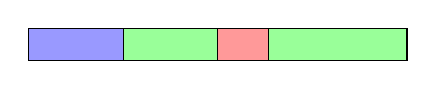
\begin{tikzpicture}[scale=0.8]
            \draw[thick] (0,2) rectangle (6,2.5);
            \draw[fill=blue!40] (0,2) rectangle (1.5,2.5);
            \draw[fill=green!40] (1.5,2) rectangle (3,2.5);
            \draw[fill=red!40] (3,2) rectangle (3.8,2.5);
            \draw[fill=green!40] (3.8,2) rectangle (6,2.5);
        \end{tikzpicture}
    \end{center}
    
    \vspace{0.2cm}
    
    \begin{block}{Nonpreemptive}
        Once a job starts, it must complete without interruption
    \end{block}
    \begin{center}
        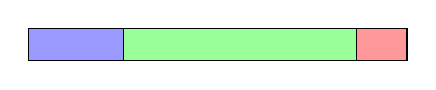
\begin{tikzpicture}[scale=0.8]
            \draw[thick] (0,2) rectangle (6,2.5);
            \draw[fill=blue!40] (0,2) rectangle (1.5,2.5);
            \draw[fill=green!40] (1.5,2) rectangle (5.2,2.5);
            \draw[fill=red!40] (5.2,2) rectangle (6,2.5);
        \end{tikzpicture}
    \end{center}
    \begin{center}
        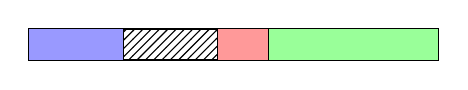
\begin{tikzpicture}[scale=0.8]
            \draw[thick] (0,-1.2) rectangle (6.5,-0.7);
            \draw[fill=blue!40] (0,-1.2) rectangle (1.5,-0.7);
            \draw[pattern=north east lines] (1.5,-1.2) rectangle (3,-0.7);
            \draw[fill=red!40] (3,-1.2) rectangle (3.8,-0.7);
            \draw[fill=green!40] (3.8,-1.2) rectangle (6.5,-0.7);
        \end{tikzpicture}
    \end{center}
    
\end{frame}

\section{The Challenge \& Strategy}

% --- Slide 3: The Challenge ---
\begin{frame}{The Challenge \& Strategy}
    \begin{columns}
        \column{0.5\textwidth}
        \textbf{Why is this hard?}
        \begin{itemize}
            \item<1-> We cannot stop a job once it starts.
            \item<2-> If a short job arrives while we are processing a long job, the short job has to wait.
            \item<3-> This is an \textbf{NP-Hard} problem.
        \end{itemize}
        
        \column{0.5\textwidth}
        \onslide<4->{
        \begin{block}{The Strategy}
            \begin{enumerate}
                \item<5-> \textbf{Relaxation:} Solve the easier \textbf{Preemptive} version first (SRPT Rule).
                \item<6-> \textbf{Rounding:} Use the completion order from the preemptive schedule.
                \item<7-> \textbf{Construction:} Schedule non-preemptively based on that order.
            \end{enumerate}
        \end{block}
        }
    \end{columns}
\end{frame}

\begin{frame}{Shortest Remaining Processing Time (SRPT)}
    \textbf{Algorithm:}
    \begin{enumerate}
        \item Start at time 0
        \item At each time, schedule the job with \textbf{smallest remaining processing time} among:
        \begin{itemize}
            \item Jobs that have been released ($t \geq r_j$)
            \item Jobs not yet completed
        \end{itemize}
        \item Continue until:
        \begin{itemize}
            \item Job completes, OR
            \item New job arrives
        \end{itemize}
        \item Repeat
    \end{enumerate}

    \vspace{0.3cm}
    \onslide<2->{
        \begin{alertblock}{Key Property}
            SRPT finds the \textbf{optimal preemptive schedule} in polynomial time!
        \end{alertblock}
    }
\end{frame}

\section{Simulation: Preemptive Scheduling}

% --- Slide 4: Example Setup ---
\begin{frame}{Simulation Example}
    Consider these 3 Jobs. We will track them through the simulation.
    
    \begin{table}
    \centering
    \begin{tabular}{lccc}
    \toprule
    \textbf{Job} & \textbf{Release ($r_j$)} & \textbf{Duration ($p_j$)} & \textbf{Visual} \\
    \midrule
    Job 1 & 0 & 2 & \textcolor{job1}{\rule{1cm}{0.3cm}} \\
    Job 2 & 1 & 5 & \textcolor{job2}{\rule{2.5cm}{0.3cm}} \\
    Job 3 & 3 & 1 & \textcolor{job3}{\rule{0.5cm}{0.3cm}} \\
    \bottomrule
    \end{tabular}
    \end{table}

    \vspace{0.5cm}
    \textbf{Step 1:} Let's run the \textbf{Preemptive} Simulation (SRPT).
\end{frame}

% --- Slide 5: Preemptive Animation ---
\begin{frame}{Simulation: Optimal Preemptive (SRPT)}
    \textbf{Rule:} Shortest Remaining Processing Time.
    
    \begin{center}
    \begin{tikzpicture}[x=1.1cm, y=1cm]
        % Base Axis (Always visible)
        \draw[->] (0,0) -- (10,0) node[right] {Time};
        \foreach \x in {0,1,...,9} \draw (\x,0.1) -- (\x,-0.1) node[below] {\x};

        % Time 0: Job 1 starts
        \onslide<2->{
            \node[anchor=south] at (0, 1.5) {\footnotesize $t=0$: J1 arrives ($p=2$). Run J1.};
            \fill[job1] (0,0.2) rectangle (2,1) node[midway, white, font=\bfseries] {J1};
        }
        
        % Time 1: Job 3 arrives decision
        \only<3>{
            \draw[red, dashed] (1, -0.5) -- (1, 2);
            \node[anchor=south, red, align=center, fill=white] at (1, 2) {
                $t=1$: J2 arrives ($p=5$). \\ 
                J1 rem = 1. \\
                $1 < 5$, so \textbf{Continue J1}.
            };
        }

        % Time 2: Job 1 finishes, Job 3 starts
        \onslide<4->{
            \node[blue, font=\bfseries] at (2,-0.8) {$C_1^P = 2$};
        }
        \onslide<5->{
            \node[anchor=south] at (5, 1.5) {\footnotesize $t=2$: J1 done. Run J2 ($p=5$).};
            \fill[job2] (2,0.2) rectangle (3,1) node[midway, white, font=\bfseries] {J2};
        }

        % Time 4: Preemption Event
        \only<6>{
            \draw[red, dashed, thick] (3, -0.5) -- (3, 2.5);
            \node[anchor=south, red, align=center, fill=white, draw=red] at (5, 2.5) {
                \textbf{INTERRUPT!} \\
                $t=3$: J3 arrives ($p=1$). \\
                J2 rem = 4 ($5-1$). \\
                $1 < 4$, so \textbf{Switch to J3}.
            };
        }

        % Time 4: Run Job 2
        \onslide<7->{
            \fill[job3] (3,0.2) rectangle (4,1) node[midway, white, font=\bfseries] {J3};
        }
        
        % Time 5: Job 2 finishes
        \onslide<8->{
            \node[red, font=\bfseries] at (4,-0.8) {$C_3^P = 4$};
            \node[anchor=south] at (6, 1) {\footnotesize $t=4$: J3 done. Resume J2.};
        }

        % Time 5: Resume Job 3
        \onslide<9->{
            \fill[job2] (4,0.2) rectangle (8,1) node[midway, white, font=\bfseries] {J2};
        }

        % Time 7: Job 3 finishes
        \onslide<10->{
            \node[green!50!black, font=\bfseries] at (8,-0.8) {$C_2^P = 8$};
        }
    \end{tikzpicture}
    \end{center}
    
    \vspace{0.5cm}
    \onslide<11->{
        \textbf{Total Completion Time:} $\sum_j C_j = 2 + 4 + 8 = \boxed{14}$ \\
        \textbf{Final Preemptive Order:} Job 1 $\to$ Job 3 $\to$ Job 2.
    }
\end{frame}

\section{2-Approximation Algorithm}

\begin{frame}{2-Approximation Algorithm for nonpreemptive scheduling}
    \begin{block}{Algorithm}
    \begin{enumerate}
        \item Find optimal preemptive schedule using SRPT
        \item Let $C_1^P \leq C_2^P \leq \cdots \leq C_n^P$ (reindex jobs by completion order)
        \item Schedule jobs \textbf{nonpreemptively} in this order:
        \begin{itemize}
            \item Job 1: from $r_1$ to $r_1 + p_1$
            \item Job 2: from $\max(r_1+p_1, r_2)$ to $\max(r_1+p_1, r_2) + p_2$
            \item Job $j$: from $\max\{C_{j-1}^N, r_j\}$ to $\max\{C_{j-1}^N, r_j\} + p_j$
        \end{itemize}
    \end{enumerate}
    \end{block}

    \vspace{0.3cm}
    \onslide<2->
    {
        \textbf{Intuition:} Jobs that finish early in preemptive schedule should finish early in nonpreemptive schedule too!
    }
\end{frame}

% --- Slide 6: The Algorithm Logic ---
\begin{frame}{2-Approximation Algorithm (contd.)}
    Now we apply this algorithm to construct the real schedule.
    
    \vspace{0.5cm}
    \begin{block}{Algorithm}
    \begin{enumerate}
        \item<1-> Sort jobs by their Preemptive Completion times ($C_j^P$).
        \item<2-> Order obtained: \textbf{1, 3, 2}.
        \item<3-> Schedule them in this \textbf{fixed order} non-preemptively.
    \end{enumerate}
    \end{block}
\end{frame}

\section{Simulation: Non-Preemptive Scheduling}

% --- Slide 7: Non-Preemptive Animation ---
\begin{frame}{Simulation: Non-Preemptive Construction}
    \textbf{Fixed Order:} 1 $\to$ 3 $\to$ 2.
    
    \begin{center}
    \begin{tikzpicture}[x=1.1cm, y=1cm]
        \draw[->] (0,0) -- (10,0) node[right] {Time};
        \foreach \x in {0,1,...,9} \draw (\x,0.1) -- (\x,-0.1) node[below] {\x};

        % Step 1: Schedule Job 1
        \onslide<2->{
            \node[anchor=south] at (1, 1.2) {\footnotesize Run J1 ($r_1=0$)};
            \fill[job1] (0,0.2) rectangle (2,1) node[midway, white, font=\bfseries] {J1};
            \node[blue, font=\bfseries] at (2, -0.8) {$C_1^N = 2$};
        }

        % Step 2: Gap for Job 2
        \only<3>{
            \node[anchor=south, red] at (6, 1.2) {Next is J3. But $r_3=3$. Wait!};
            \fill[idle] (2,0.2) rectangle (3,1) node[midway, black] {Idle};
        }
        
        % Step 3: Run Job 2
        \onslide<4->{
            \fill[idle] (2,0.2) rectangle (3,1) node[midway, black] {Idle};
            \fill[job3] (3,0.2) rectangle (4,1) node[midway, white, font=\bfseries] {J3};
            \node[red, font=\bfseries] at (4, -0.8) {$C_3^N = 4$};
        }

        % Step 4: Run Job 3
        \only<5>{
            \node[anchor=south] at (7, 1.2) {Next is J2 ($r_2=1$). Ready to go!};
        }
        \onslide<6->{
            \fill[job2] (4,0.2) rectangle (9,1) node[midway, white, font=\bfseries] {J2};
            \node[green!50!black, font=\bfseries] at (9, -0.8) {$C_2^N = 9$};
        }
        
    \end{tikzpicture}
    \end{center}
    
    \vspace{0.5cm}
    \onslide<7->{
        Total Completion Time: $2 + 4 + 9 = \boxed{15}$.
    }
\end{frame}

\section{Observation 4.1}

\begin{frame}{Observation 4.1}
    \begin{block}{Observation 4.1}
    $$\sum_{j=1}^{n} C_j^P \leq \text{OPT}$$
        where $C_j^P$ is completion time in optimal preemptive schedule and OPT is optimal nonpreemptive objective.
    \end{block}

    \vspace{0.5cm}
    \textbf{Proof:}
    \begin{itemize}
        \item<2-> Any nonpreemptive schedule is also a valid preemptive schedule
        \item<3-> The optimal preemptive schedule is at least as good as any preemptive schedule
        \item<4-> Therefore, optimal preemptive $\leq$ optimal nonpreemptive
    \end{itemize}
\end{frame}

\section{Lemma 4.2: Bounding the Delay}

\begin{frame}{Lemma 4.2: Bounding the Delay}
    \begin{block}{Lemma 4.2}
        For each job $j = 1, \ldots, n$: \quad $C_j^N \leq 2C_j^P$ \\
    \end{block}
    Here jobs are indexed according to the ascending order of their completion time.

    \vspace{0.3cm}
    \onslide<2->{
        \textbf{Proof Idea:} We'll show $C_j^N$ cannot be too large by using two lower bounds on $C_j^P$.
        
        \vspace{0.3cm}
        \textbf{Lower Bounds on $C_j^P$:}
    }

    \begin{enumerate}
        \item<3-> \textbf{Release dates:} Job $j$ cannot complete before any of jobs $1, \ldots, j$ are released:
        $$C_j^P \geq \max_{k=1,\ldots,j} r_k$$
        
        \item<4-> \textbf{Processing times:} Jobs $1, \ldots, j$ need time to process:
        $$C_j^P \geq \sum_{k=1}^{j} p_k$$
    \end{enumerate}
\end{frame}

\begin{frame}{Lemma 4.2: Upper Bound on $C_j^N$}
    \textbf{Key Observation:} In nonpreemptive schedule, machine is idle only when waiting for next job's release.

    \vspace{0.3cm}
    \onslide<2->{
        \begin{center}
            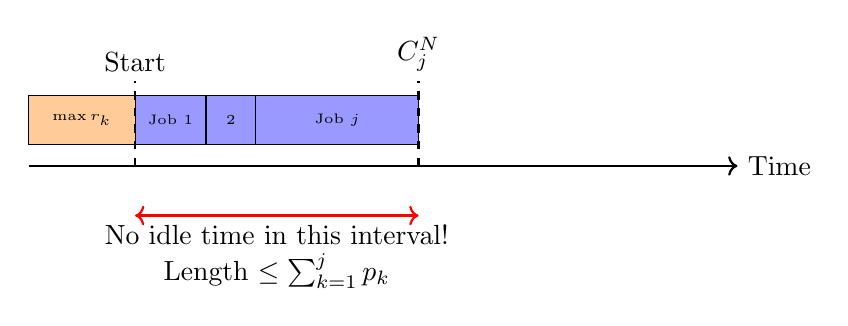
\begin{tikzpicture}[scale=0.9]
                \draw[thick,->] (0,0) -- (10,0) node[right] {Time};

                % Max release date
                \draw[fill=orange!40] (0,0.3) rectangle (1.5,1);
                \node at (0.75,0.65) {\tiny $\max r_k$};
                \draw[dashed,thick] (1.5,0) -- (1.5,1.2);
                \node[above] at (1.5,1.2) {Start};

                % Processing
                \draw[fill=blue!40] (1.5,0.3) rectangle (2.5,1);
                \node at (2,0.65) {\tiny Job 1};
                \draw[fill=blue!40] (2.5,0.3) rectangle (3.2,1);
                \node at (2.85,0.65) {\tiny 2};
                \draw[fill=blue!40] (3.2,0.3) rectangle (5.5,1);
                \node at (4.35,0.65) {\tiny Job $j$};

                % No idle time
                \draw[<->,thick,red] (1.5,-0.7) -- (5.5,-0.7);
                \node[below] at (3.5,-0.7) {No idle time in this interval!};
                \node[below] at (3.5,-1.1) {Length $\leq \sum_{k=1}^j p_k$};

                \draw[dashed,thick] (5.5,0) -- (5.5,1.2);
                \node[above] at (5.5,1.2) {$C_j^N$};
            \end{tikzpicture}
        \end{center}
    }
    \vspace{0.2cm}
    onslide<3->{
        Therefore: $C_j^N \leq \max_{k=1,\ldots,j} r_k + \sum_{k=1}^{j} p_k$
    }
\end{frame}

\begin{frame}{Lemma 4.2: Completing the Proof}
    We have:
    \begin{align*}
        C_j^N &\leq \max_{k=1,\ldots,j} r_k + \sum_{k=1}^{j} p_k \\
        &\leq C_j^P + C_j^P \quad \text{(using both lower bounds)} \\
        &= 2C_j^P
    \end{align*}

    \vspace{0.5cm}
    \begin{center}
        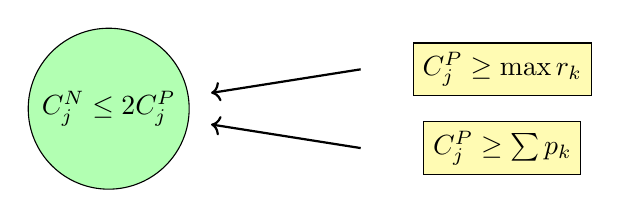
\begin{tikzpicture}
            \node[draw,circle,fill=green!30,minimum size=2cm] at (0,0) {$C_j^N \leq 2C_j^P$};
            \node[draw,rectangle,fill=yellow!30] at (5,0.5) {$C_j^P \geq \max r_k$};
            \node[draw,rectangle,fill=yellow!30] at (5,-0.5) {$C_j^P \geq \sum p_k$};
            \draw[->,thick] (3.2,0.5) -- (1.3,0.2);
            \draw[->,thick] (3.2,-0.5) -- (1.3,-0.2);
        \end{tikzpicture}
    \end{center}
    onslide<2->{
        \textbf{Result:} Each job's completion time at most doubles! \qed
    }
\end{frame}

\section{Theorem 4.3: The Result}

\begin{frame}{Theorem 4.3: The Result}
    \begin{block}{Theorem 4.3}
        Scheduling in order of the completion times of an optimal preemptive schedule is a \textbf{2-approximation algorithm} for scheduling a single machine with release dates to minimize the sum of completion times.
    \end{block}

    \vspace{0.5cm}
    \textbf{Proof:}
    \onslide<2->{
        \begin{align*}
            \sum_{j=1}^{n} C_j^N &\leq 2\sum_{j=1}^{n} C_j^P \quad \text{(by Lemma 4.2)} \\
            &\leq 2 \cdot \text{OPT} \quad \text{(by Observation 4.1)}
        \end{align*}
    }

    \vspace{0.3cm}
    \onslide<3->{
        \begin{center}
            \boxed{\text{Our algorithm's cost} \leq 2 \times \text{Optimal cost}}
        \end{center}
    }
\end{frame}

\section{Summary}

\begin{frame}{Key Takeaways}
    \begin{enumerate}
        \item<1-> \textbf{Problem:} Schedule $n$ jobs on single machine nonpreemptively to minimize $\sum C_j$
        
        \vspace{0.3cm}
        \item<2-> \textbf{SRPT Rule:} Optimal algorithm for preemptive version (always schedule job with shortest remaining processing time)
        
        \vspace{0.3cm}
        \item<3-> \textbf{Our Algorithm:}
        \begin{itemize}
            \item Find optimal preemptive schedule
            \item Schedule jobs nonpreemptively in same completion order
        \end{itemize}
        
        \vspace{0.3cm}
        \item<4-> \textbf{Result:} 2-approximation algorithm
        \begin{itemize}
            \item Uses two key bounds: release dates and total processing time
            \item Each job's completion time at most doubles
        \end{itemize}
    \end{enumerate}
\end{frame}

\begin{frame}{Visual Summary}
    \begin{center}
        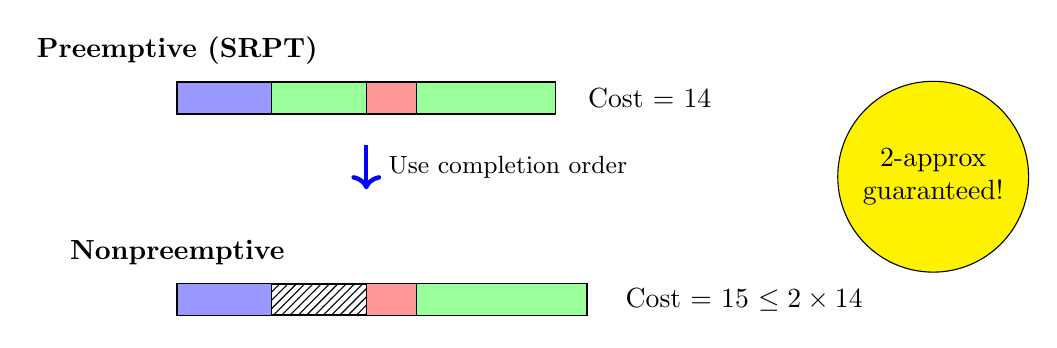
\begin{tikzpicture}[scale=0.8]
            % Preemptive
            \node at (0,3) {\textbf{Preemptive (SRPT)}};
            \draw[thick] (0,2) rectangle (6,2.5);
            \draw[fill=blue!40] (0,2) rectangle (1.5,2.5);
            \draw[fill=green!40] (1.5,2) rectangle (3,2.5);
            \draw[fill=red!40] (3,2) rectangle (3.8,2.5);
            \draw[fill=green!40] (3.8,2) rectangle (6,2.5);
            \node at (7.5,2.25) {Cost = 14};

            % Arrow
            \draw[->,ultra thick,blue] (3,1.5) -- (3,0.8);
            \node[right] at (3.2,1.15) {\small Use completion order};

            % Nonpreemptive
            \node at (0,-0.2) {\textbf{Nonpreemptive}};
            \draw[thick] (0,-1.2) rectangle (6.5,-0.7);
            \draw[fill=blue!40] (0,-1.2) rectangle (1.5,-0.7);
            \draw[pattern=north east lines] (1.5,-1.2) rectangle (3,-0.7);
            \draw[fill=red!40] (3,-1.2) rectangle (3.8,-0.7);
            \draw[fill=green!40] (3.8,-1.2) rectangle (6.5,-0.7);
            \node at (9,-0.95) {Cost = 15 $\leq 2 \times 14$};

            \node[draw,circle,fill=yellow,text width=2cm,align=center] at (12,1) {2-approx guaranteed!};
        \end{tikzpicture}
    \end{center}
\end{frame}

% --- Slide 12: Questions ---
\begin{frame}
    \centering
    \Huge \textbf{Any Questions?}
\end{frame}

% --- Slide 13: Thank You ---
\begin{frame}
    \centering
    \vspace{1cm}
    \Huge \textcolor{blue}{Thank You!}
    
    \vspace{1cm}
    \large
    \textbf{Presenter:} Tanvir Hossain \\
    \small Student ID: 2005014
\end{frame}

\end{document}